    \section{Filtr Notcha o częstotliwości 50 Hz}

    \subsection{Schemat filtra}
xxxxxxxxx
% --- photo: filtr nr 1 ---
\begin{figure}[H]
\centering
\setlength{\fboxrule}{2pt}
\setlength{\fboxsep}{0pt}
\fbox{
    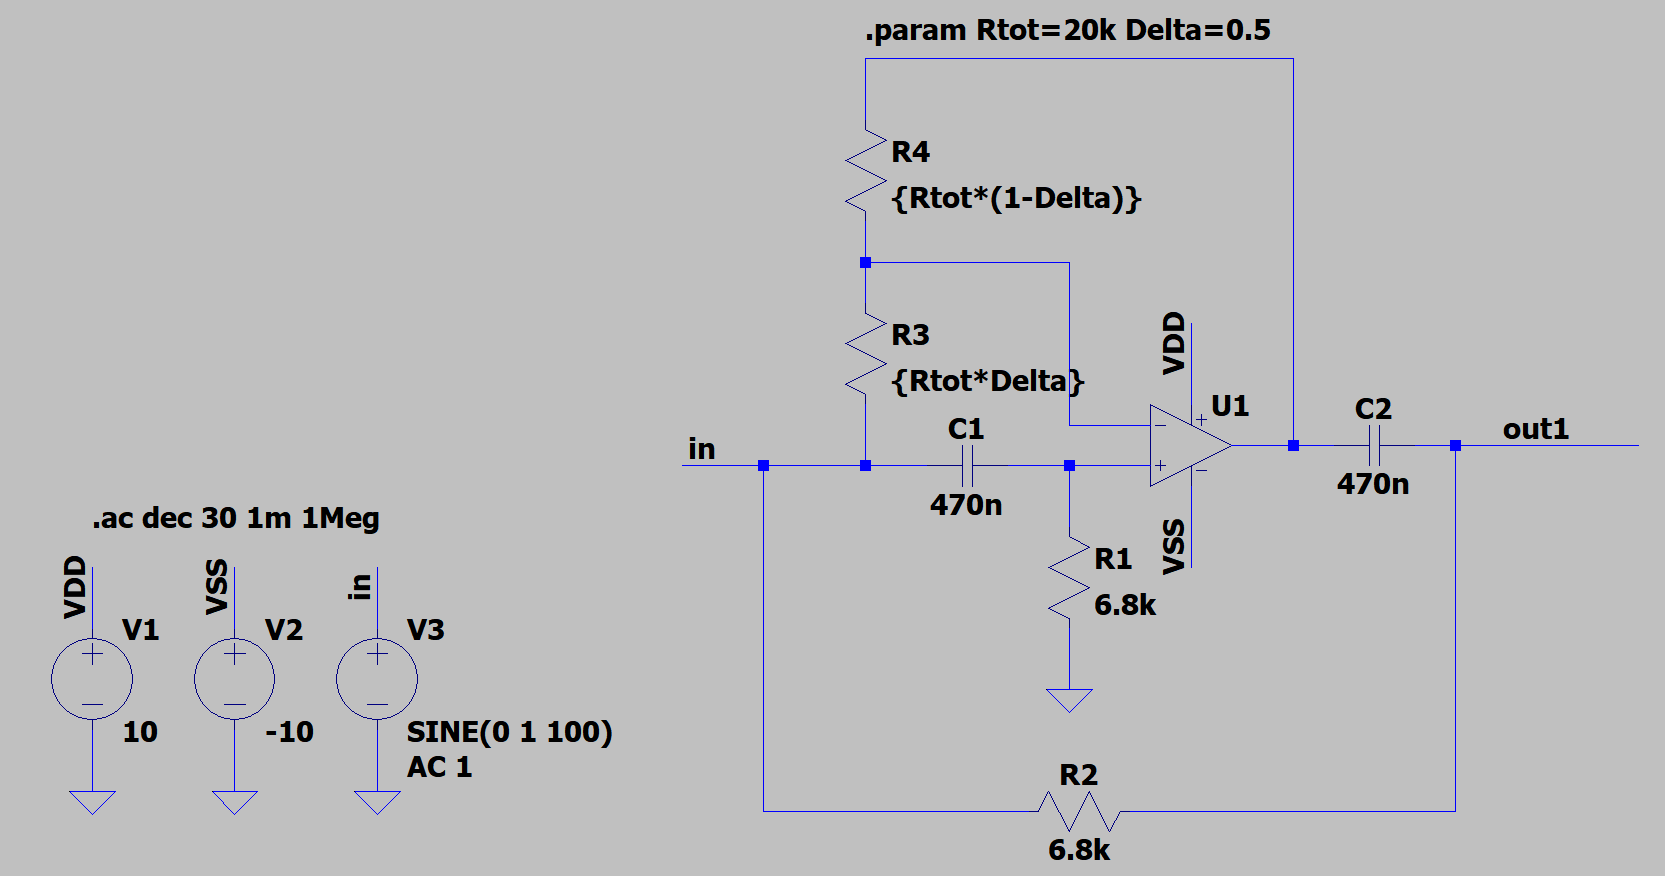
\includegraphics[width=1\textwidth]{figures/NotchF_ideal.png}
}
\caption{Uproszczony schemat projektowanego filtru Notcha.}
\end{figure}
% --- end photo ---

    \subsection{Wartości użytych elementów}

    \subsubsection{Wartości teoretyczne}
xxxxxxxxxxxxxxx\\
xxxxxxxxxxxxxxx
\begin{itemize}
    \item R1 = R2 = 6.8 k$\Omega$
    \item C1 = C2 = 470 nF
\end{itemize}
Wszystkie te wartości są naniesione na schemacie filtra w podsekcji 4.1.

    \subsubsection{Wartości rzeczywiste}
Rzeczywiste wartości elementów różnią się nieznacznie od teoretycznych i
wynoszą:
\begin{itemize}
    \item R1 = 6.74 k$\Omega$
    \item R2 = 6.70 k$\Omega$
    \item C1 = C2 = 470 nF
\end{itemize}
    \subsection{Odpowiedź częstotliwościowa filtra}

    \subsubsection{Symulacja}
Symulując filtr Notcha w programie LTspice uzyskaliśmy poniższą 
charakterystykę, na której można zauważyć tłumienie na poziomie
44 decybeli sygnału o częstotliwości bliskiej 50 Hz.
% --- photo: freq response Notcha ---
\begin{figure}[H]
\centering
\setlength{\fboxrule}{2pt}
\setlength{\fboxsep}{0pt}
\fbox{
    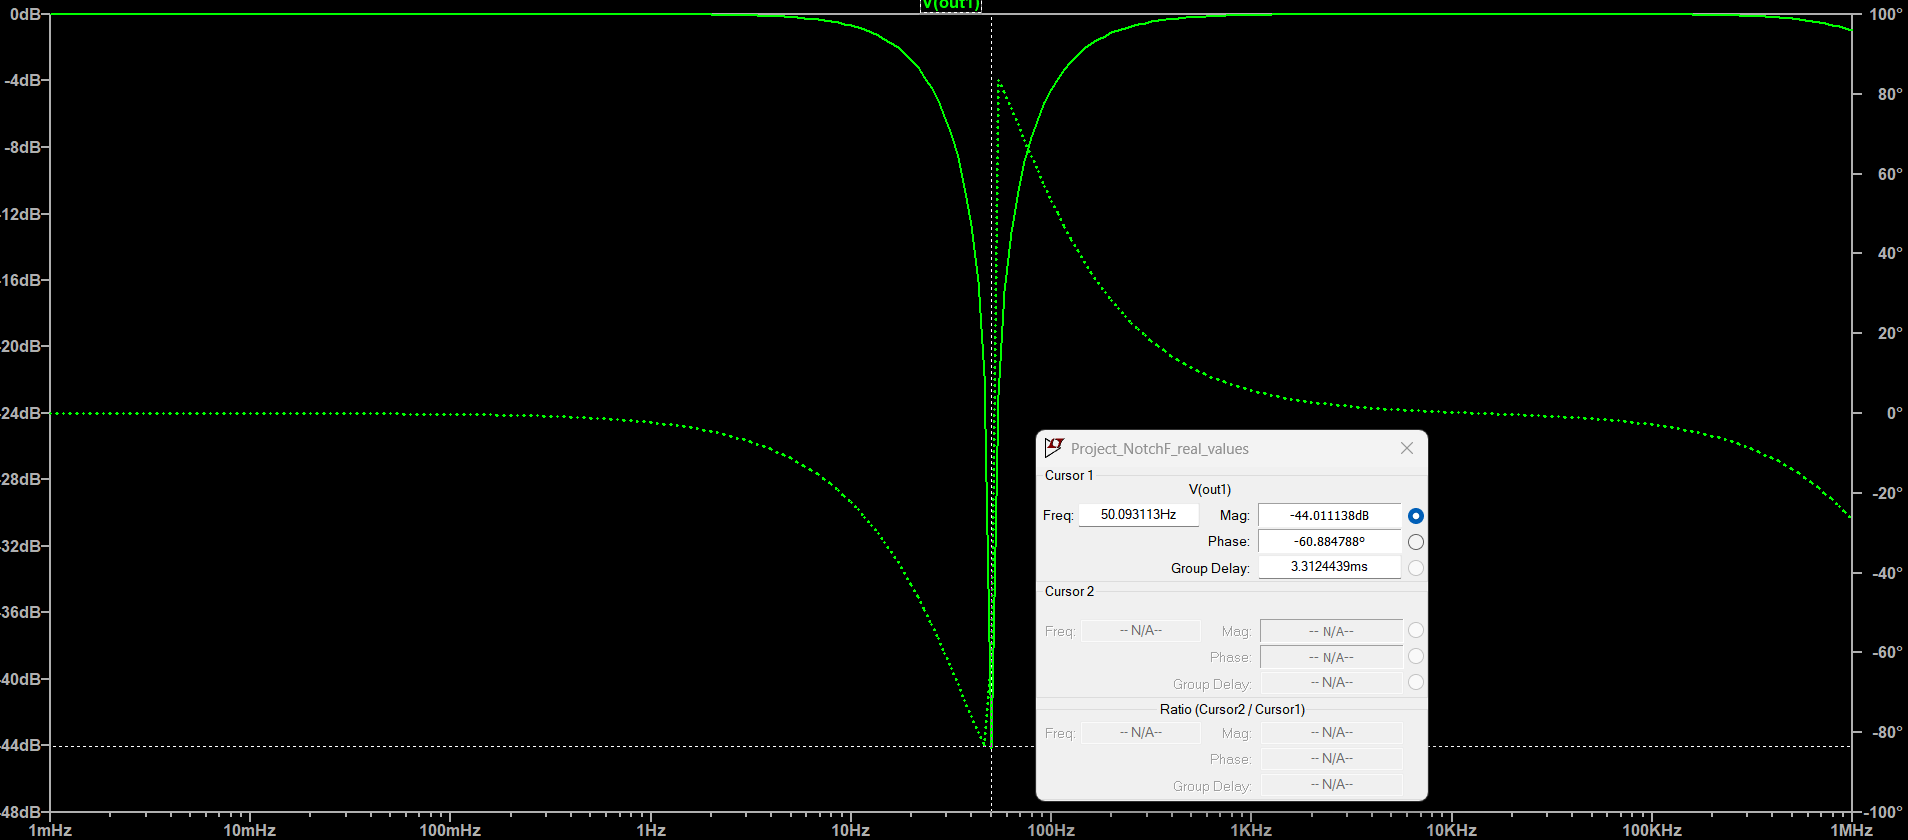
\includegraphics[width=1\textwidth]{plots/NotchF_freq_response.png}
}
\caption{Odpowiedź częstotliwościowa filtru Notcha.}
\end{figure}
% --- end photo ---

    \subsubsection{Pomiary}
No trzeba by było zrobić żeby coś tu wpisać\ldots